\newpage
	\section{MAGNETOMETRO}
	Un magnetómetro\autoref{fig:MAG} es un dispositivo capaz de identificar la dirección de referencia, normalmente el norte, a partir de la medición del campo magnético de la tierra.
	Existen\cite{ScienceDirect_Magnetometer} diferentes tipos de magnetómetros, el más sencillo es la brújula magnética, la cual rastrea la orientación de una aguja metálica dentro del campo magnético de la tierra.como se puede arpeciar en \cite{TransducerResearch_Magnetoresistive} Esta tiene ciertos problemas, como el que el norte magnético de la tierra no se alinea con el norte geográfico, necesitando entonces calibrar según la ubicación para considerar este desfase. Otro problema es que son fácilmente influenciadas por otras fuentes de campos magnéticos. 
		\begin{figure}[h]
		\centering
		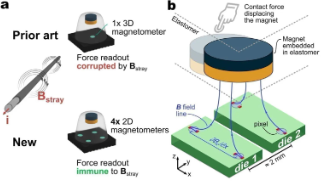
\includegraphics[width=0.3\linewidth]{img/MAG}
		\caption{Magnetometro }
		\label{fig:MAG}
	\end{figure}
	
	Las brújulas electrónicas pueden encontrar el norte magnético a partir de propiedades electrónicas. Estas normalmente utilizan el efecto Hall para su medición, aunque algunas utilizan el efecto magneto-resistivo.

	El efecto Hall se basa en las propiedades electromagnéticas de ciertos materiales, por ejemplo, si suministramos corriente a través de una placa metálica la cual a continuación se le aplica un campo magnético, dentro de la placa se distorsionara su campo eléctrico, por lo que un lado de la placa se cargará negativamente y el otro positivamente. Midiendo con un voltímetro las cargas de la placa podemos determinar que tan fuerte es el campo magnético.
	El efecto magneto-resistivo basa su funcionamiento en el hecho que ciertos materiales pueden cambiar su resistividad si son expuestos a un campo magnético.
	
	\section{LiDAR}
El LiDAR\autoref{fig:LiDAR} es un sensor que utiliza láseres para medir distancias, movimientos de un entorno, calcular superficies y mapear un espacio señalado \cite{IBM_Lidar}.
\begin{figure}[h]
	\centering
	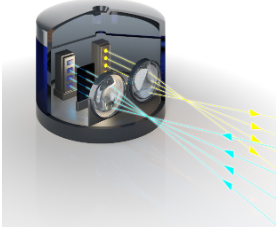
\includegraphics[width=0.3\linewidth]{img/LiDAR}
	\caption{Magnetometro }
	\label{fig:LiDAR}
\end{figure}

\section*{Tipos de sensores LiDAR:}
\begin{itemize}
	\item Topográfico 
	\item Batimétrico  
\end{itemize}




